\section{Information Architecture}

\subsection{Organisation Structures}
Our web application has Hybrid Organization Structure. In this type of organization structure there is a relation between hierarchical model and database. We are planning to use this type of organization since in our system, there is a hierarchy between the web pages and there should be a database system in it. The web pages should have a relation to a database. 

\begin{figure}[h!]
  \centering  
  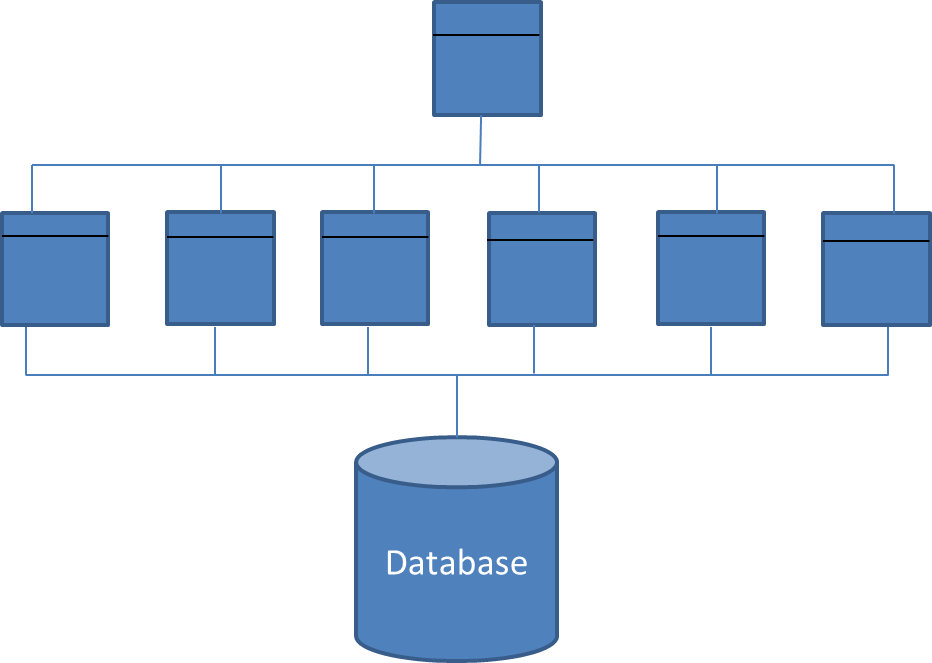
\includegraphics[width=0.5\textwidth]{Images/hybrid_org.png}                
  \caption{Hybrid Organisation Structure}
  \label{fig:hybrid_org}
\end{figure}


\subsection{Organisation Schemes}
Our system has Inexact Organisation Schemes. The users are able to find the items by means of topic. It is beneficial for particularly the first time users who may not know what they are searching. This scheme provides to a subject searching. 

\subsection{Labelling Systems}
We aim to develop a user-friendly web application, therefore it is important to have specific and clear labels. To determine the labels which are used in our web application, we look through some websites selling baby clothes such as oshkoshbgosh.com and babymallonline.com.

\begin{itemize}
\item In our application, there are a reasonable number of categories. 
\item Each category has some members. 
\item In order to determine the labels, we analyzed the results of the queries which we did.
\end{itemize}

We have different groups for baby boys and baby girls so that these two groups have some different type of clothes. The users generally try to find an item by means of the type of the clothes, so we have labels of different type of baby clothes. We reached this result after analyzing the questionnaire results. Also there are two other labels which are clearance and second hand, users are able to look through these pages in order to find some cheaper items.
We use some other subgroups under the main groups so that user be able to find the items they wanted.. These labels are tops, bottoms, footwear . Under these subgroups, users can look through the type of clothes.

\subsubsection{Labels}
\begin{itemize}
\setlength{\itemsep}{-3pt}
\setlength{\parskip}{0pt}
\setlength{\parsep}{0pt}
 \item Boy 
 \item Girl 
 \item Clearance 
 \item Second Hand
\end{itemize}

\minisec{Boy}
\begin{itemize}
\setlength{\itemsep}{-3pt}
\setlength{\parskip}{0pt}
\setlength{\parsep}{0pt}

	 \item Tops
	 	\begin{itemize}
\setlength{\itemsep}{-3pt}
\setlength{\parskip}{0pt}
\setlength{\parsep}{0pt}
		 \item Shirts and Tees
      	 \item Jackets
      	 \item Sweaters and Hoodies
		\end{itemize}
     \item Bottoms
	 	\begin{itemize}
\setlength{\itemsep}{-3pt}
\setlength{\parskip}{0pt}
\setlength{\parsep}{0pt}
		 \item Trousers
		 \item Jeans
		 \item Shorts
		\end{itemize}
	 \item Footwear
	 	\begin{itemize}
\setlength{\itemsep}{-3pt}
\setlength{\parskip}{0pt}
\setlength{\parsep}{0pt}
		 \item Boots
		 \item Sneakers
		 \item Sandals
		 \item Socks
		\end{itemize}
	 \item Bodysuits	
     \item Pajamas
	\end{itemize}

\minisec{Girl} 
\begin{itemize}
\setlength{\itemsep}{-3pt}
\setlength{\parskip}{0pt}
\setlength{\parsep}{0pt}

	 \item Tops (same as for Boy)
     \item Bottoms
	 	\begin{itemize}
\setlength{\itemsep}{-3pt}
\setlength{\parskip}{0pt}
\setlength{\parsep}{0pt}
		 \item Trousers
		 \item Jeans
		 \item Shorts
		 \item Skirts
		\end{itemize}
	 \item Dresses 
	 \item Footwear (same as for Boy)
	 \item Bodysuits	
     \item Pajamas
	\end{itemize}
\minisec{Clearance and Second Hand} 
\begin{itemize}
\setlength{\itemsep}{-3pt}
\setlength{\parskip}{0pt}
\setlength{\parsep}{0pt}

	 \item Tops
	 	\begin{itemize}
\setlength{\itemsep}{-3pt}
\setlength{\parskip}{0pt}
\setlength{\parsep}{0pt}
		 \item Shirts and Tees
      	 \item Jackets
      	 \item Sweaters and Hoodies
		\end{itemize}
     \item Bottoms
	 	\begin{itemize}
\setlength{\itemsep}{-3pt}
\setlength{\parskip}{0pt}
\setlength{\parsep}{0pt}
		 \item Trousers
		 \item Jeans
		 \item Shorts
		 \item Skirts
		\end{itemize}
	 \item Dresses
	 \item Footwear
	 	\begin{itemize}
\setlength{\itemsep}{-3pt}
\setlength{\parskip}{0pt}
\setlength{\parsep}{0pt}
		 \item Boots
		 \item Sneakers
		 \item Sandals
		 \item Socks
		\end{itemize}
	 \item Bodysuits	
     \item Pajamas
	\end{itemize}

